%%
% Please see https://bitbucket.org/rivanvx/beamer/wiki/Home for obtaining beamer.
%%
\documentclass{beamer}
\usepackage{amsmath,amsbsy,amsopn,amstext,amsfonts,amssymb}
\usepackage{isomath}
\usepackage{ulem}
%\linespread{1.6}  % double spaces lines
\usepackage{graphicx}
\usepackage{subfigure}
\usepackage{color}
\usepackage{optidef}  % define optimization problems
\usepackage{multicol}  % multiple columns
\usepackage{listings} % for python code
\usepackage{mathrsfs}

\usepackage{polynom}
\newcommand{\adj}{\mathrm{adj}}
\newcommand{\constrainedmin}[3]{
		\begin{mini*}|s|
		{#2}{#1}{}{}
		\addConstraint{#3}
		\end{mini*}
}

\newcommand{\rwbcomment}[1]{{\color{blue}RWB:#1}}
\newcommand{\defeq}{\stackrel{\triangle}{=}}
\newcommand{\abs}[1]{\left|#1\right|}
\newcommand{\norm}[1]{\left\|#1\right\|}
\newcommand{\iprod}[1]{\left<#1\right>}
\newcommand{\ellbf}{\boldsymbol{\ell}}
\newcommand{\nubf}{\boldsymbol{\nu}}
\newcommand{\mubf}{\boldsymbol{\mu}}
\newcommand{\abf}{\mathbf{a}}
\newcommand{\bbf}{\mathbf{b}}
\newcommand{\cbf}{\mathbf{c}}
\newcommand{\dbf}{\mathbf{d}}
\newcommand{\ebf}{\mathbf{e}}
\newcommand{\fbf}{\mathbf{f}}
\newcommand{\gbf}{\mathbf{g}}
\newcommand{\hbf}{\mathbf{h}}
\newcommand{\ibf}{\mathbf{i}}
\newcommand{\jbf}{\mathbf{j}}
\newcommand{\kbf}{\mathbf{k}}
\newcommand{\lbf}{\mathbf{l}}
\newcommand{\mbf}{\mathbf{m}}
\newcommand{\nbf}{\mathbf{n}}
\newcommand{\obf}{\mathbf{o}}
\newcommand{\pbf}{\mathbf{p}}
\newcommand{\qbf}{\mathbf{q}}
\newcommand{\rbf}{\mathbf{r}}
\newcommand{\sbf}{\mathbf{s}}
\newcommand{\tbf}{\mathbf{t}}
\newcommand{\ubf}{\mathbf{u}}
\newcommand{\vbf}{\mathbf{v}}
\newcommand{\wbf}{\mathbf{w}}
\newcommand{\xbf}{\mathbf{x}}
\newcommand{\ybf}{\mathbf{y}}
\newcommand{\zbf}{\mathbf{z}}
\newcommand{\Jbf}{\mathbf{J}}
\newcommand{\Acal}{\mathcal{A}}
\newcommand{\Bcal}{\mathcal{B}}
\newcommand{\Lcal}{\mathcal{L}}
\newcommand{\Ncal}{\mathcal{N}}
\newcommand{\Rcal}{\mathcal{R}}
\definecolor{darkolivegreen}{rgb}{0.33, 0.42, 0.18}

\makeatletter
\newenvironment<>{proofstart}[1][\proofname]{%
    \par
    \def\insertproofname{#1\@addpunct{.}}%
    \usebeamertemplate{proof begin}#2}
  {\usebeamertemplate{proof end}}
\newenvironment<>{proofcont}{%
  \setbeamertemplate{proof begin}{\begin{block}{}}
    \par
    \usebeamertemplate{proof begin}}
  {\usebeamertemplate{proof end}}
\newenvironment<>{proofend}{%
    \par
    \pushQED{\qed}
    \setbeamertemplate{proof begin}{\begin{block}{}}
    \usebeamertemplate{proof begin}}
  {\popQED\usebeamertemplate{proof end}}
\makeatother

\title{ECEn 671: Mathematics of Signals and Systems \\ 
Moon: Chapter 2.}
\author{Randal W. Beard}
\institute{Brigham Young University}
\date{\today}

\begin{document}

%-------------------------------
\begin{frame}
	\titlepage
\end{frame}

%-------------------------------
\begin{frame}[t]
\frametitle{Table of Contents}
\tableofcontents
\end{frame}

%%%%%%%%%%%%%%%%%%%%%%%%%%%%%%%%%%%%%%%%%%%%%%%%%%%%%%%%%%%%%%%%%%%%%%%
\section{Metric Spaces}
\frame{\sectionpage}

%----------------------------------
\begin{frame}\frametitle{Spaces}

\begin{itemize}
\item One of the objectives of this course is to develop tools that work in a wide variety of settings.  
\item We will mostly focus on \underline{finite dimensional Hilbert spaces}, which include:
	\begin{itemize}
		\item $\mathbb{R}^n$, $\mathbb{C}^n$, $\mathbb{C}^{m\times n}$,
		\item the set of all functions with finite integral,
		\item the set of all finitely summable sequences,
		\item binary vectors, binary sequences.
	\end{itemize}
\item But does not include important objects like 
	\begin{itemize}
	\item rotations matrices, quaternions, homogeneous transformations.	
	\end{itemize}
\item To make things clear, we will develop the theory systematically in the following order:
	\begin{enumerate}
		\item Metric space
		\item Norm space / Banach space
		\item Inner product space / Hilbert space
	\end{enumerate}
\end{itemize}
\end{frame}

%----------------------------------
\begin{frame}\frametitle{Metric Spaces}

\begin{definition}[Metric Space] A \underline{metric space} is a pair $(\mathbb{X},d)$ where $\mathbb{X}$ is a set and 
	\[
	d:\mathbb{X} \times \mathbb{X} \to \mathbb{R}
	\]
	is a metric defined over $\mathbb{X}$.\\
\end{definition}
	
A metric is a measure of distance between elements in a set.
\end{frame}

%----------------------------------
\begin{frame}\frametitle{Metric Spaces}
\begin{definition}[Metric]
Let $\mathbb{X}$ be a set.  Then 
$d:\mathbb{X} \times \mathbb{X} \to \mathbb{R}$ is a metric if:

\begin{align*} 
(M1) \qquad & d(x,y) = d(y,x), \quad \forall x,y \in \mathbb{X} \\
(M2) \qquad & d(x,y) \geq 0, \quad \forall x,y \in \mathbb{X} \\
(M3) \qquad & d(x,y) = 0, \quad \iff x = y\\
(M4) \qquad &d(x,z) \leq d(x,y) + d(y,z), \quad \forall x,y,z \in \mathbb{X}
\end{align*}
\end{definition}

(M4) is called the \underline{Triangle inequality}.
\end{frame}

%----------------------------------
\begin{frame}\frametitle{Examples of Metric Spaces}

\begin{example}[E1]

$(\mathbb{R}, d)$ where $d(x,y) \defeq |x-y|$ is a metric space.

Note that 
\begin{itemize}
	\item (M1) $|x-y| = |y-x|$, $\forall x,y \in \mathbb{R}$.
	\item (M2) $|x-y|\geq 0$, $\forall x,y \in \mathbb{R}$.	
	\item (M3) $|x-y| = 0$, if $x=y$.	
	\item (M4) $|x-z|\leq |x-y| + |y-z|$ $\forall x,y,z \in \mathbb{R}$. 
\end{itemize}
\end{example}

To convince yourself (M4), draw a picture.  Note, a picture is not a proof.

\end{frame}

%----------------------------------
\begin{frame}\frametitle{Examples of Metric Spaces}

\begin{example}[E2]

$(\mathbb{R}^n, d)$ where 
\[
d(x,y) \defeq \left( \sum_{i=1}^{n} |x_i - y_i|^2 \right)^{\frac{1}{2}}
\]
where $x=(x_1, \dots, x_n)^\top$ and $y=(y_1, \dots, y_n)^\top$.

Verify that $d(\cdot, \cdot)$ satisfies (M1)-(M4).
\end{example}
\end{frame}

%----------------------------------
\begin{frame}\frametitle{Examples of Metric Spaces}

\begin{example}[E3]

$(\mathbb{R}^n, d)$ where 
\[
d(x,y) \defeq \left( \sum_{i=1}^{n} |x_i - y_i|^p \right)^{\frac{1}{p}}
\]
where $p\geq 1$.

For general $p\geq 1$, the triangle inequality is a nontrivial and famous results.
\end{example}

\end{frame}

%----------------------------------
\begin{frame}\frametitle{Examples of Metric Spaces}

\begin{example}[E4 bounded sequence space]

Let $\boldsymbol{\ell}^\infty$ be the set of all sequences of complex numbers where each number is bounded, i.e., 
\[
x = (x_1, x_2, x_3, \dots) \in \boldsymbol{\ell}
\]
if $x_i\in\mathbb{C}$ and $\abs{x_i}<\infty$.

$(\boldsymbol{\ell}, d)$ is a metric space where
\[
d(x, y) = \sup_{j\in\mathbb{N}} \abs{x_i - y_i}.
\]
\end{example}

Verify (M1)-(M4).
\end{frame}

%----------------------------------
\begin{frame}\frametitle{Examples of Metric Spaces}

\begin{example}[E5 continuous function space]
\begin{itemize}
\item Let $C[a,b]$ be the set of all continuous functions on $[a,b]$, i.e., \\
\indent \indent i.e. $ x \in C[a,b] \Rightarrow x(t) $ is continuous on $[a,b]$.\\
Let 
\[ 
d(x,y) = \max_{t \in [a,b]} |x(t)-y(t)| 
\]
then $(C[a, b], d)$ is a metric space.

\item This is a different perspective than calculus.  In calculus you consider one function at a time.  In this class, a function is one \underline{point} in a larger metric space.
\end{itemize}
\end{example}
\end{frame}

%----------------------------------
\begin{frame}\frametitle{Examples of Metric Spaces}

\begin{example}[E6 discrete metric space]

Let $\mathbb{X}$ be any set, e.g., the set of three legged dogs, and let
\[
d(x,y) = \begin{cases}
 1 & \text{~if~} x\neq y \\
 0 & \text{~otherwise}	
 \end{cases}.
 \]
 Then $(\mathbb{X}, d)$ is a metric space since
\begin{itemize}
	\item (M1) $d(x,y) = d(y,x)$, $\forall x,y \in \mathbb{X}$.
	\item (M2) $d(x,y) \geq 0$, $\forall x,y \in \mathbb{X}$.	
	\item (M3) $d(x,y) = 0$, if $x=y$.	
	\item (M4) $d(x,z)\leq d(x,y) + d(y,z)$ $\forall x,y,z \in \mathbb{X}$. 
\end{itemize}
\end{example}
\end{frame}

%----------------------------------
\begin{frame}\frametitle{Examples of Metric Spaces}

\begin{example}[E7 binary vector space]

Let $\mathbb{X}=\{0,1\}^n$ be the set of binary vectors, i.e \\
$x\in\mathbb{X} \Rightarrow x=(x_1, x_2, \dots, x_n)$ where $x_i\in \{0, 1\}$.
Let 
\[ 
d(x,y) = \sum_{i=1}^{n}{h(x_i - y_i)} 
\]  
where
\[ 
h(w) = \begin{cases} 
	1 & \text{ if } \qquad w \neq 0 \\ 
	0 & \text{ otherwise }
\end{cases}.
\]
$h$ is called the hamming distance, and simply counts the number of elements in $x$ and $y$ that are different.
\end{example}
\end{frame}

%----------------------------------
\begin{frame}\frametitle{Metric Spaces / Norm Spaces / Inner Product Spaces}

\begin{itemize}
\item Later in the chapter, 	we will later introduce the concepts of a norm and a norm space, and an inner product and inner product spaces.
\item Many of the metric spaces introduced above are also norm spaces and inner product spaces, but not all.  
\item Metric spaces are the most general of the three.  
\item Before introducing the concept of a norm and a normed space, we develop general tools that also work for metric spaces.
\end{itemize}
\end{frame}

%%%%%%%%%%%%%%%%%%%%%%%%%%%%%%%%%%%%%%%%%%%%%%%%%%%%%%%%%%%%%%%%%%%%%%%
\section{Topology}
\frame{\sectionpage}

%----------------------------------
\begin{frame}\frametitle{Topology}

\begin{itemize}
\item In this next section, we develop a set of tools that fall under that category of \underline{topology}.  
\item These tools hold for metric spaces (including norm and inner product spaces).
\item WARNING:  There are a lot of definitions.  These definitions will help talk formally about things in the future.
\end{itemize}
\end{frame}

%----------------------------------
\begin{frame}\frametitle{Topology: Open and Closed Sets}

\begin{definition}[Ball] Given a metric space $(\mathbb{X},d)$ a $\delta$-ball around $x_0$ is defined to be
\(
B(x_0,\delta) = \{ x \in \mathbb{X} : d(x,x_0) < \delta \}
\)
\end{definition}
\begin{definition}[Interior Point]
 A point $x_o \in \mathbb{X}$ is interior to $S \subset \mathbb{X}$ if 
\(
\exists \delta > 0 \text{ such that } B(x_o,\delta) \subset S.
\)
\end{definition}
\begin{definition}[Open Set] A set $\mathbb{X}$ is \underline{open} if all points in $\mathbb{X}$ are interior.	
\end{definition}

\begin{definition}[Closed Set] A set $S$ is closed in $\mathbb{X}$ if $\mathbb{X}\setminus S$ is open.	
\end{definition}

\end{frame}

%----------------------------------
\begin{frame}\frametitle{Topology: Convergence}

Let $(\mathbb{X},d)$ be a metric space.

\begin{definition}[Convergence] Given a sequence $\{x_n\}_{n=1}^\infty$, where $x_n\in\mathbb{X}$, the following are equivalent
\begin{itemize}
  \item $\lim_{n \to \infty} x_n = x^*$
  \item $x_n \rightarrow x^*$
  \item $\forall \epsilon > 0, \exists N(\epsilon) \text{ such that } n \geq N \Rightarrow d(x_n,x^*) < \epsilon$
\end{itemize}
A sequence $\{x_n\}_{n=1}^\infty$ in $\mathbb{X}$ with a limit $x^\ast \in \mathbb{X}$ is said to converge.
\end{definition}
\end{frame}

%----------------------------------
\begin{frame}\frametitle{Topology: Convergence}

Note that a limit may not always exist (similar to min, max)
    
    For example, $\lim_{t\to\infty}sin(t)$ does not exist. \\
   
\begin{definition}[$\lim\sup$] Define $\lim \sup$ as the largest limit (possibly infinity) of any subsequence.	
\end{definition}
\begin{definition}[$\lim\inf$]
Define $\lim \inf$ is the smallest limit of all possible subsequences.
\end{definition}

\begin{example}
\begin{itemize}
\item $\underset{t\to\infty}{\lim\sup} \enspace \sin(t) = 1 $ since the subsequence $t_n = \frac{k\pi}{2}, k = 1,5,9,\cdots$ converges to 1
\item $\underset{t\to\infty}{\lim\inf} \enspace \sin(t) = -1 $ since the subsequence $t_n = \frac{k\pi}{2}, k = 3,7,11,\cdots$ converges to -1
\end{itemize}
\end{example}
\end{frame}

%----------------------------------
\begin{frame}\frametitle{Topology: Cauchy Sequence}

\begin{definition}[Cauchy Sequence]
A sequence $\{x_n\}_{n=1}^\infty$ in a metric space $(\mathbb{X},d)$ is said to be a Cauchy sequence if $\forall \epsilon > 0 , \exists N(\epsilon) > 0$ such that $n,m > N \Rightarrow d(x_n,x_m) < \epsilon$
\end{definition}

A sequence is Cauchy if elements in its tail get increasingly closer together.  Note that we have not said anything about an element of convergence.

\begin{theorem} If a sequence $\{x_n\}_{n=1}^\infty$ in $\mathbb{X}$ converges to an element $x^\ast\in\mathbb{X}$ then it is a Cauchy sequence.  	
\end{theorem}


The converse is not true!!  I.e., not all Cauchy sequences converge.  
\end{frame}


%----------------------------------
\begin{frame}\frametitle{Topology: Cauchy Sequence}

\begin{example}[from book]
Let $\mathbb{X} = C[-1,1]$ and $d(f,g) = \left( \displaystyle\int_{-1}^{1}{(f(t) - g(t))^2dt} \right)^{\frac{1}{2}}$\\
let $f_n:$

\begin{center}
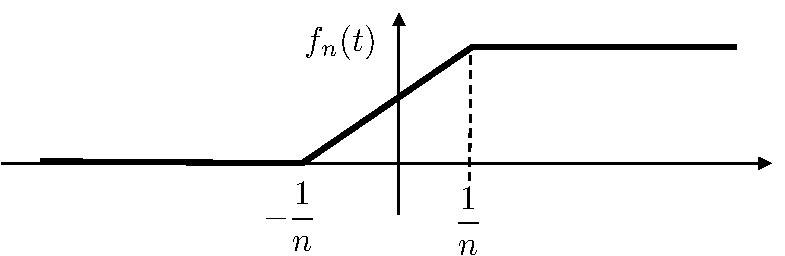
\includegraphics[width=0.6\textwidth]{figures/chap2_discontinuous_function}\\
\end{center}

By integration we get:
\[ d(f_n,f_n) = \frac{1}{6m^3n}(m^3+4m^2n + mn^2 + 2n^3) \]
\[\to 0 \text{ for } n,m \text{ large } (m > n) \]
but $f_n$ converges to a discontinuous function which is not in $\mathbb{X}$.  This is undesirable.
\end{example}
\end{frame}

%----------------------------------
\begin{frame}\frametitle{Topology: Complete Metric Space}

\begin{definition}[Complete metric space]
A metric space $(\mathbb{X},d)$ is \underline{complete} if every Cauchy sequence in $\mathbb{X}$ converges to a value in $\mathbb{X}$.\\
\end{definition}

\begin{block}{Implication}
 $C[a,b]$ with metric $(\int_{a}^{b}\abs{f-g}^2 dt)^{1/2}$ is \underline{not} complete.	
\end{block}

\begin{itemize}
\item Banach spaces are \underline{complete} normed spaces (discussed later).
\item Hilbert spaces (extremely important in signal processing and control) are complete inner product spaces (discussed later).
\item The importance of $L_p$ and $\ell_p$ are that they are complete spaces.
\end{itemize}

%$\rightarrow$ Notes on $L_p$:\\
%
%\quad $x \in L_p$ is actually a family of functions not a single function.  The following functions are equivalent:\\
%\includegraphics[width=0.9\textwidth]{chap2imgs/1-page6}\\
%
%In fact equivalent functions can differ at a countable infinite number of points!\\
%
%Technically they can differ on a set of measure zero.  All functions with the same Lebesque integral are said to be equivalent.\\
\end{frame}

%%%%%%%%%%%%%%%%%%%%%%%%%%%%%%%%%%%%%%%%%%%%%%%%%%%%%%%%%%%%%%%%%%%%%%%
\section{Vector Spaces}
\frame{\sectionpage}

%----------------------------------
\begin{frame}\frametitle{Vector Spaces}


\subsection*{Definition: Field} A \underline{field} is a set of scalars with well defined addition and multiplication operations.

{\bf Example of fields:}  
\begin{itemize}
\item $\mathbb{R}$ with normal addition and multiplication operations
\item $\mathbb{C}$ with complex addition and complex multiplication
\item The set of quaternions, with addition and quaternion multiplication
\item Binary numbers $\{0, 1\}$ where addition is the ``or'' operator and multiplication is the ``and'' operator.
\end{itemize}
\end{frame}

%----------------------------------
\begin{frame}\frametitle{Vector Spaces}

\begin{definition}[Linear Vector Space] A \underline{linear vector space} is a pair $(\mathbb{X},\mathbb{F})$, where  $\mathbb{X}$ is a set of objects, and $\mathbb{F}$ is a field, this is closed under addition and scalar multiplication. i.e., \\
\begin{itemize}
\item $x\in\mathbb{X}, \alpha \in \mathbb{F} \Rightarrow \alpha x \in \mathbb{X}$
\item $x,y \in \mathbb{X} \Rightarrow x+y\in\mathbb{X}$.
\end{itemize}
\end{definition}
By implication
\begin{itemize}
\item $x\in\mathbb{X}, \alpha,\beta\in\mathbb{F} \Rightarrow (\alpha + \beta)x = \alpha x + \beta x \in \mathbb{X}$
\item $x,y\in\mathbb{X}, \alpha\in\mathbb{F} \Rightarrow \alpha(x + y) = \alpha x + \alpha y \in\mathbb{X}$
\item $x,y\in\mathbb{X}, \alpha,\beta\in\mathbb{F} \Rightarrow \alpha x + \beta y \in \mathbb{X}$.
\end{itemize}
\end{frame}

%----------------------------------
\begin{frame}\frametitle{Vector Spaces: Subspace}

\begin{definition}[Subspace] A \underline{subspace} $V \subset \mathbb{X}$ is a subset of $\mathbb{X}$ that is also a linear vector space, in particular it contains zero.	
\end{definition}


\par\noindent{\bf Important property:} A vector space contains a \underline{zero} element.	

\end{frame}

%----------------------------------
\begin{frame}\frametitle{Vector Spaces: Examples}


The following are vector spaces:
\begin{itemize}
\item $(\mathbb{R}^n, \mathbb{R})$, $(\mathbb{C}^n, \mathbb{C})$, $(\mathbb{R}^{m\times n}, \mathbb{R})$, $(C[a,b], \mathbb{R})$, $(\boldsymbol{\ell}^\infty, \mathbb{R})$, $(L^\infty, \mathbb{R})$.
\end{itemize}

The following are NOT vector spaces:
\begin{itemize}
\item 	The set $\mathbb{X}=\mathbb{R} \times [0,2\pi]$, (a cylinder) is not a vector space for any field $\mathbb{F}$.  This is the state space for an inverted pendulum.
\item The set of rotation matrices is not a vector space for any field $\mathbb{F}$.   This is in the configuration space for robots and satellites.\\
\item The set of unit quaternions is not a vector space for any field.  Quaternions are used extensively in robotics, quantum mechanics, and computer graphics.
\item There are many useful spaces that are NOT linear vector spaces.
\end{itemize}
\end{frame}

%----------------------------------
\begin{frame}\frametitle{Vector Spaces: Linear Independence}


Let $S$ be a vector space and let $T \subset S$.  ($T$ may have uncountable infinite members).  $T$ is linearly independent if for each \underline{finite} nonempty subset of $T$. i.e., $\{p_1,\cdots,p_n\}$ where $p_i\in T$, we have that 
\[
c_1p_1+\cdots+c_np_n=0 \qquad \iff \quad c_1=c_2=\cdots=c_n=0.
\]
Otherwise $T$ is linearly dependent.
\end{frame}

%----------------------------------
\begin{frame}\frametitle{Vector Spaces: Linear Independence}

\begin{example}  Let $S=\mathbb{R}^3$ then the set $T=\{ (1,0,0)^\top, (0, 1, 0)^\top \} \subset \mathbb{R}^3$ is linearly independent since
\[
c_1\begin{pmatrix} 1 \\ 0 \\ 0 \end{pmatrix} + c_2\begin{pmatrix} 0 \\ 1 \\ 0 \end{pmatrix} = \begin{pmatrix} c_1 \\ c_2 \\ 0 \end{pmatrix} = \begin{pmatrix} 0 \\ 0 \\ 0 \end{pmatrix}
\]
if and only if $c_1=c_2=0$.  

However, the set $T=\{ (1,1,0)^\top, (2, 2, 0)^\top \} \subset \mathbb{R}^3$ is linearly dependent since
\[
c_1\begin{pmatrix} 1 \\ 1 \\ 0 \end{pmatrix} + c_2\begin{pmatrix} 2 \\ 2 \\ 0 \end{pmatrix} = \begin{pmatrix} c_1+2c_2 \\ c_1+2c_2 \\ 0 \end{pmatrix} = \begin{pmatrix} 0 \\ 0 \\ 0 \end{pmatrix}
\]
when $c_1=-2$ and $c_2=1$ (as only on example).
\end{example}
\end{frame}

%----------------------------------
\begin{frame}\frametitle{Vector Spaces: Span}

\begin{definition}[Span]
	Let $S$ be a vector space, then $\text{span}(T)$ is the set of all linear combinations of $T\subseteq S$.
\end{definition}
 
\begin{example} 
\[
\text{span}\left\{ \left( \begin{array}{c} 1 \\ 1 \end{array} \right) \right\} = \left\{ \begin{pmatrix} \alpha \\ \alpha \end{pmatrix} | \alpha\in\mathbb{R} \right\}
\]
\end{example}
\begin{example} 
\[
\text{span}\left\{ \left( \begin{array}{c} 1\\0 \end{array}\right),\left(\begin{array}{c}0\\1\end{array}\right)\right\}= \left\{\begin{pmatrix} \alpha \\ \beta \end{pmatrix}:\alpha, \beta\in\mathbb{R}\right\} = \mathbb{R}^2.
\]
\end{example}
\end{frame}

%----------------------------------
\begin{frame}\frametitle{Vector Spaces: Basis}

\begin{definition}[Basis] $T$ is a \underline{basis} for the vector space $S$ if $T$ is linearly independent and $\mathrm{span}(T)=S$.	
\end{definition}

\begin{definition}[Dimension] The dimension of the vector space $S$ is the smallest number of linearly independent vectors needed to span $S$.	
\end{definition}

\begin{example}
One possible basis for $\mathbb{R}^n$ is given by
\[
\left\{\left(\begin{array}{c}1\\0\\\vdots\\0\end{array}\right),\left(\begin{array}{c}0\\1\\\vdots\\0\end{array}\right)\cdots,\left(\begin{array}{c}0\\0\\\vdots\\1\end{array}\right)\right\}.
\]
Therefore $\dim(\mathbb{R}^n) = n$.
\end{example}
\end{frame}

%----------------------------------
\begin{frame}\frametitle{Vector Spaces: Basis}

\begin{example}
One possible basis for $\boldsymbol{\ell}^\infty$ is given by
\[
\left\{
  \left(
    \begin{array}{c}
      1\\
      0\\
      0\\
      \vdots\\
      \vdots\\
      \vdots
    \end{array}
  \right)
  ,\left(
    \begin{array}{c}
      0\\
      1\\
      0\\
      \vdots\\
      \vdots\\
      \vdots
    \end{array}
  \right)
  ,\cdots,
  \left(
    \begin{array}{c}
      0\\
      0\\
      \vdots\\
      0\\
      1\\
      0\\
      \vdots
    \end{array}
  \right)
  ,\cdots
\right\}
\]
Therefore $\dim(\boldsymbol{\ell}^\infty) = \infty$.
\end{example}
\end{frame}

%----------------------------------
\begin{frame}\frametitle{Vector Spaces: Basis}
\begin{example}
The set of all polynomials $P$ is a vector space with basis
\[ \{1,t,t^2,\cdots\} \]
Therefore $\dim(P) = \infty$.
\end{example}

\begin{example}
The set of all polynomials of degree $\leq q$ $P^q$ is a vector space with basis
\[ \{1,t,t^2,\cdots, t^q\} \]
Therefore $\dim(P^q) = q$.
\end{example}
\end{frame}

%%%%%%%%%%%%%%%%%%%%%%%%%%%%%%%%%%%%%%%%%%%%%%%%%%%%%%%%%%%%%%%%%%%%%%%
\section{Normed Spaces}
\frame{\sectionpage}

%----------------------------------
\begin{frame}\frametitle{Norms and Normed Spaces}
\begin{definition}[Norm] Let $S$ be a vector space, $\norm{ x }$ is a norm if:
\begin{flalign*}
(N1) \qquad & \norm{ x } \geq 0 \quad \forall x \in S\\
(N2) \qquad & \norm{ x } = 0 \quad \Leftrightarrow x = 0\\
(N3) \qquad & \norm{ \alpha x } = \alpha\norm{ x }\\
(N4) \qquad & \norm{ x + y } \leq \norm{ x } + \norm{ y }\quad \text{(triangle inequality)}\\
\end{flalign*}
\end{definition}
\end{frame}

%----------------------------------
\begin{frame}\frametitle{Differences between norms and metrics:}
\begin{itemize}
\item Norms only have one argument (the length of a vector), where metrics are distances between elements of a set.
\item Norms are only defined for vector spaces!\\
(i.e. there is no norm for rotation matrices, but there are metrics!)
\item Norms scale with the vector (N3)\\
(there are metrics that don't scale), e.g. $d(x,y) = \begin{cases} 1 \quad x &\neq y\\0 \quad x &= y\end{cases}$
\item Every norm is also a metric\\
\[ \norm{ x - y } = d(x,y) \]
\[ \norm{ x } = d(x,0) \]
\end{itemize}
\end{frame}

%----------------------------------
\begin{frame}\frametitle{Definition: Normed Space} 

A \underline{normed} space is a pair $(\mathbb{X},\norm{ \cdot} )$ where $\mathbb{X}$ is a vector space and $\norm{ \cdot} $ is a norm.

\begin{example}[Normed Spaces]
$\mathbb{R}^n$ is a vector space.  All of the following norms are valid:
\begin{itemize}
  \item one-norm \quad $\norm{ x}_1 = \displaystyle \sum_{i=1}^{n}|x_i|$ \quad (power vectors)
  \item two-norm \quad $\norm{ x}_2 = \displaystyle \left( \sum_{i=1}^{n}|x_i|^2 \right)^{\frac{1}{2}}$ \quad (energy vectors)
  \item infinity-norm \quad $\norm{ x}_{\infty} = \underset{i=1,\cdots,n}{\max}|x_i|$ \quad (bounded vectors)
  \item p-norm \quad $\norm{ x}_p = \left( \displaystyle \sum_{i=1}^{n}|x_i|^p \right)^{\frac{1}{p}}$
\end{itemize}
\end{example}
\end{frame}

%----------------------------------
\begin{frame}\frametitle{Unit Circle in $\mathbb{R}^2$}

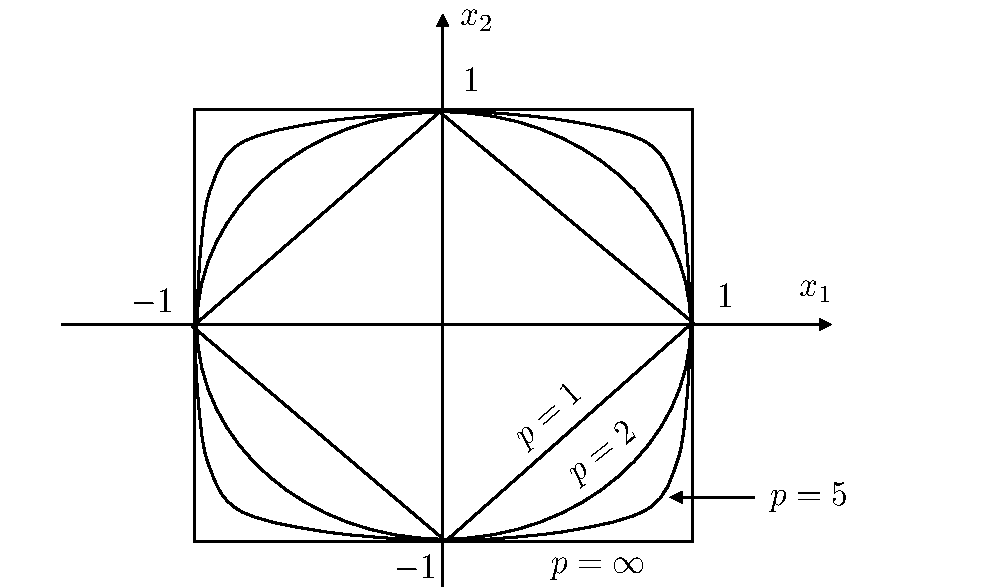
\includegraphics[width=0.9\textwidth]{figures/chap2_unit_circle}\\
	
\end{frame}
 

%----------------------------------
\begin{frame}\frametitle{Normed Space Example: Sequence Spaces}
Let $\boldsymbol{\ell}$ be the set of sequences: $x = (x_1, x_2, x_3, \cdots)$.  
The following normed vector spaces can be defined:
\begin{itemize}
\item $\boldsymbol{\ell}_1$: (power sequences)  If $\norm{ x}_{\ell_1} = \sum_{i=1}^{\infty}|x_i|$ then 
$\boldsymbol{\ell}_1 \defeq \{x \in \boldsymbol{\ell} : \norm{x}_{\ell_1} < \infty \}$
\item $\boldsymbol{\ell}_2$: (energy sequences)  If $\norm{ x}_{\ell_2} = \left(\sum_{i=1}^{\infty}|x_i|^2\right)^{1/2}$ then $\boldsymbol{\ell}_2 \defeq \{x \in \boldsymbol{\ell} : \norm{x}_{\ell_2} < \infty \}$
\item $\boldsymbol{\ell}_\infty$: (bounded sequences)  If $\norm{ x}_{\ell_\infty} = \sup_{j\in\mathbb{N}}|x_j|$ then $\boldsymbol{\ell}_\infty \defeq \{x \in \boldsymbol{\ell} : \norm{x}_{\ell_\infty} < \infty \}$
\item $\boldsymbol{\ell}_p$:  If $\norm{ x}_{\ell_p} = \left(\sum_{i=1}^{\infty}|x_i|^p\right)^{1/p}$ then $\boldsymbol{\ell}_p \defeq \{x \in \boldsymbol{\ell} : \norm{x}_{\ell_p} < \infty \}$ for $1\leq p \leq\infty$
\end{itemize}
\end{frame}

%----------------------------------
\begin{frame}\frametitle{Normed Space Examples}

\begin{example}
Consider the sequence $x = (1,1,1,\ldots)$:
\begin{itemize}
\item $x \in \boldsymbol{\ell}_{\infty}$, but
\item $x \notin \boldsymbol{\ell}_p \text{ for } 1 \leq p < \infty$.
\end{itemize}
\end{example}

\begin{example}
Consider the sequence $x = (1, \frac{1}{2}, \frac{1}{3}, \frac{1}{4}, \ldots)$
\begin{itemize}
\item 	$x \notin \boldsymbol{\ell}_1$ (prove this), but 
\item $x \in \boldsymbol{\ell}_p \quad p > 1$ (prove this)
\end{itemize}
\end{example}
\end{frame}

%----------------------------------
\begin{frame}\frametitle{Normed Space Example: Function Spaces}
Let $L^n(\Omega)$ be the set of functions on $\Omega$. $x\in L^n(\Omega)$ is an equivalent classes of functions, i.e. equal except on a set of measure zero.  (picture)  The following norms are valid:
\begin{itemize}
\item 	$L_1^n(\Omega)$ (power signals).  If $\norm{x}_{L_1^n(\Omega)} = \int_{\Omega}\norm{ x(t)}  dt$, then $L_1^n(\Omega) = \{ x\in L^n(\Omega)| \norm{x}_{L_1^n(\Omega)} < \infty \}$.
\item $L_2^n(\Omega)$ (energy signals).  If $\norm{x}_{L_2^n(\Omega)} = \left(\int_{\Omega}\norm{ x(t)}^2  dt\right)^{1/2}$, then $L_2^n(\Omega) = \{ x\in L^n(\Omega)| \norm{x}_{L_2^n(\Omega)} < \infty \}$.
\item $L_p^n(\Omega)$.  If $\norm{x}_{L_p^n(\Omega)} = \left(\int_{\Omega}\norm{ x(t)}^p  dt\right)^{1/p}$, then $L_p^n(\Omega) = \{ x\in L^n(\Omega)| \norm{x}_{L_p^n(\Omega)} < \infty \}$, $1\leq p \leq \infty$.
\item 	$L_\infty^n(\Omega)$ (bounded signals).  If $\norm{x}_{L_\infty^n(\Omega)} = \sup_{t\in\Omega}\norm{ x(t)}$, then $L_\infty^n(\Omega) = \{ x\in L^n(\Omega)| \norm{x}_{L_\infty^n(\Omega)} < \infty \}$.
\end{itemize}
\end{frame}

%%%%%%%%%%%%%%%%%%%%%%%%%%%%%%%%%%%%%%%%%%%%%%%%%%%%%%%%%%%%%%%%%%%%%%%
\section{Inner Product Spaces}
\frame{\sectionpage}

%----------------------------------
\begin{frame}\frametitle{Inner Product Spaces}
\begin{definition}[Inner Product] Let $S$ be a vector space over $\mathbb{R}$.  An inner product $<\cdot,\cdot>:S \times S \to \mathbb{R}$ has the following properties:\\
\begin{flalign*}
(IP1) \qquad &\iprod{x,y} = \overline{\iprod{ y,x }}\\
(IP2) \qquad &\iprod{\alpha x,y} = \alpha \iprod{ x,y }\\
(IP3) \qquad &\iprod{ x+y,z } = \iprod{ x,z } + \iprod{ y, z }\\
(IP4) \qquad &\iprod{ x,x } > 0 \quad \text{~if~} x \neq 0, \iprod{ x,x}=0 \Leftrightarrow x=0
\end{flalign*}
\end{definition}

\begin{definition}[Inner Product Space] A vector space with an inner product defined is called an inner-product space.	
\end{definition}

\begin{definition}[Hilbert Space] A complete inner-product space is called a \underline{Hilbert space}.	
\end{definition}

\end{frame}

%----------------------------------
\begin{frame}\frametitle{Inner Product Spaces: Examples}
\begin{itemize}
	\item $\mathbb{R}^n$: $\iprod{ x,y } = \sum_{i=1}^{n} x_i y_i = x^Ty$ is called the Euclidean inner product.
	\item $\mathbb{C}^n$: $\iprod{ x,y } = \sum_{i=1}^{n} x_i \overline{y_i} = y^Hx$
\end{itemize}
\begin{itemize}
	\item $\mathbb{R}^n$ with the Euclidean inner product is a Hilbert space	.
	\item $\mathbb{C}^n$ with the Euclidean inner product is a Hilbert space.
	\item All finite-dimensional inner-product spaces are Hilbert spaces.
\end{itemize}
\end{frame}
	
%----------------------------------
\begin{frame}\frametitle{Inner Product Spaces: Examples}
\begin{itemize}
	\item Real sequences $\boldsymbol{\ell}_2 $: $\iprod{ x,y }_{\ell_2} = \sum_{i=1}^{\infty} x_i y_i$
	\item Complex sequences $\boldsymbol{\ell}_2$:  $\iprod{ x,y }_{\ell_2} = \sum_{i=1}^{\infty} x_i \overline{y_i}$
	\item Both of these examples are Hilbert spaces.
\end{itemize}
\end{frame}

%----------------------------------
\begin{frame}\frametitle{Inner Product Spaces: Examples}
\begin{itemize}
	\item Complex function space $L_2^n(\Omega)$ with inner product:
		\[
		\iprod{ x,y } = \displaystyle \int_{\infty} y^H(t)x(t) \,dt
		\]
		is a Hilbert space, but 
	\item Continuous function $C[a,b]$ with the same inner product is NOT a Hilbert space.
\end{itemize}
\end{frame}

%----------------------------------
\begin{frame}\frametitle{Norms vs Inner Products}
Every inner product defines a norm (but not vice-versa)
\[ 
\norm{ x}  = \iprod{ x,x }^{\frac{1}{2}} 
\] 
where $\norm{\cdot}$ is called the norm induced by the inner product $\iprod{\cdot, \cdot}$.
\end{frame}

%----------------------------------
\begin{frame}\frametitle{Examples of inducted norms}

\begin{flalign*}
\norm{ \cdot}_2\text{:  }\iprod{ x,x }^{1/2} &= \left( \displaystyle \sum_{i=1}^{n}x_i^2 \right)^{1/2} = \norm{ x}_2\\
\norm{ \cdot}_{\ell_2}\text{:  }\iprod{ x,x }^{1/2} &= \left( \displaystyle \sum_{i=1}^{\infty} x_i^2 \right)^{1/2} = \norm{ x}_{\ell_2}\\
\norm{ \cdot}_{L_2}\text{:  }\iprod{ x,x }^{1/2} &= \left( \displaystyle \int_{\Omega} x^T(t)x(t) dt \right)^{1/2}
= \left( \int_{\Omega} \norm{ x(t)}_2^2 dt \right)^{1/2}
= \norm{ x}_{L_2}\\
\end{flalign*}

Note that induced norms are all $2-$norms.
\end{frame}

%----------------------------------
\begin{frame}\frametitle{Cauchy-Schwartz Inequality}
\begin{theorem}[Cauchy-Schwartz]
Let $S$ be any inner product space (doesn't need to be Hilbert) and let $\norm{ \cdot}  = \iprod{ \cdot, \cdot }^{1/2}$\\
then $\forall x,y \in S$
\[ |\iprod{ x,y } | \leq \norm{ x}  \norm{ y}  \]
with equality iff $y=\alpha x$ where $\alpha\in\mathbb{F}$ is any scalar in the field $\mathbb{F}$.
\end{theorem}
\end{frame}

%----------------------------------
\begin{frame}\frametitle{Cauchy-Schwartz Inequality: Proof}
The inequality clearly holds if either $x=0$ or $y=0$.  Therefore assume that $x \neq 0$ and $y \neq 0$. Then
\begin{align*}
	\norm{ x-\alpha y} ^2 &= \iprod{ x-\alpha y, x - \alpha y } \\
		&=\iprod{ x ,x } - \alpha \iprod{ y,x } - \iprod{ x, \alpha y } + \iprod{ \alpha y, \alpha y } \\
		&=\iprod{ x ,x } - \alpha \iprod{ y,x } - \overline{\overline{\iprod{ x, \alpha y }}} + \alpha \overline{\overline{\iprod{ y, \alpha y }}} \\
		&=\iprod{ x ,x } - \alpha \iprod{ y,x } - \overline{\iprod{ \alpha y, x }} + \alpha \overline{\iprod{ \alpha y, y }} \\
		&=\iprod{ x ,x } - \alpha \iprod{ y,x } - \overline{\alpha} \overline{\iprod{ y, x }} + \alpha\overline{\alpha}\overline{\iprod{ y, \alpha y }}\\
		&=\iprod{ x ,x } - \alpha \iprod{ y,x } - \overline{\alpha} \iprod{ x, y } + \abs{\alpha}^2\iprod{ y, y } \\
		&=\norm{x}^2 - \alpha \iprod{ y,x } - \overline{\alpha} \iprod{ x, y } + \abs{\alpha}^2\norm{y}^2 \\
\end{align*}
\end{frame}

%----------------------------------
\begin{frame}\frametitle{Cauchy-Schwartz Inequality: Proof}
Recall the technique of completing the square:
\begin{flalign*}
ax^2+bx+c &= a(x^2 + \frac{b}{a}x) + c\\
&= a(x+\frac{b}{2a})^2 - \frac{b}{4a}^2 + c.
\end{flalign*}
Complete the square in $\alpha$:
\begin{align*}
\norm{ x-\alpha y}^2 &= \norm{ y} ^2 \left(\alpha\overline{\alpha} - \alpha \frac{\overline{ \iprod{ x,y } }}{\norm{ y} ^2} - \bar\alpha \frac{\iprod{ x,y }}{\norm{ y} ^2} \right) + \norm{ x} ^2 \\
	&= \norm{ y} ^2 \left( \alpha - \frac{\iprod{ x,y }}{\norm{ y} ^2}\right)\left(\bar\alpha - \frac{\overline{\iprod{ x,y }}}{\norm{ y} ^2}\right) - \frac{|\iprod{ x,y } |^2}{\norm{ y} ^2} + \norm{ x} ^2
\end{align*}
\end{frame}

%----------------------------------
\begin{frame}\frametitle{Cauchy-Schwartz Inequality: Proof}
Let $\alpha^*= \frac{\iprod{ x,y }}{\norm{ y} ^2}$ to get
\begin{align*}
	& 0 \leq \norm{ x - \alpha^*y} ^2 = \norm{ x} ^2 - \frac{|\iprod{ x,y }|^2}{\norm{ y} ^2} \\
	\Rightarrow &\qquad |\iprod{ x,y } |^2 \leq \norm{ x} ^2\norm{ y} ^2 \\
	\Rightarrow &\qquad |\iprod{ x,y } | \leq \norm{ x}  \norm{ y}
\end{align*}
\end{frame}

%%%%%%%%%%%%%%%%%%%%%%%%%%%%%%%%%%%%%%%%%%%%%%%%%%%%%%%%%%%%%%%%%%%%%%%
\section{Notions of Convergence}
\frame{\sectionpage}

%----------------------------------
\begin{frame}\frametitle{Notions of Convergence}

\begin{definition}[Strong Convergence/ Convergence in norm]
$x_n$ converges strongly to $x$, i.e. $x_n \overset{s}{\to} x$ iff
\[
\norm{ x_n-x}  \to 0 \quad \mathit{ as } \quad n \to \infty 
\]	
\end{definition}

\begin{definition}[Weak Convergence / Convergence in inner product]
$x_n$ converges weakly to $x$, i.e. $x_n \overset{w}{\to} x$ iff
\[ 
\iprod{ x_n, y } \to \iprod{ x,y }, \forall y \in S, 
\]	
\end{definition}

Note that this must hold for all $y \in S$, therefore Example 2.4.4 in the book is bogus!

\end{frame}

%----------------------------------
\begin{frame}\frametitle{Notions of Convergence (cont.)}
\begin{theorem}[Strong vs. Weak Convergence]
  Let $(x_n)$ be a sequence in a normed space $\mathbb{X}$.  Then
\begin{description}
  \item[A.] Strong convergence $\Rightarrow$ weak convergence with the same limit
  \item[B.] The converse of (A.) is not generally true
  \item[C.] If dim $\mathbb{X} < \infty$, then weak convergence $\Rightarrow$ strong convergence.
\end{description}
\end{theorem}
	
\end{frame}

%----------------------------------
\begin{frame}\frametitle{Proof:}
\noindent (A) By definition of strong convergence,
\[ 
x_n \overset{s}{\to} x^* \quad \Rightarrow \quad \norm{ x_n-x^*}  \to 0
\]
so let $y$ be \underline{any} element in $\mathbb{X}$ then
\[ 
|\iprod{ x_n,y } - \iprod{ x^*,y } | = |\iprod{ x_n - x^*,y } | \leq \norm{ x_n-x^*}  \norm{ y}  
\]
but the RHS $\to 0$ which implies that the LHS $\to 0$ which implies weak convergence.
\end{frame}

%----------------------------------
\begin{frame}\frametitle{Proof:}
\noindent (B) Before proving part (B) lets first understand what is wrong with Example 2.4.4 in the book.
\begin{align*}
x_n &= (0,0,0,\ldots,1,0,\ldots) \\
y &= (1, 1/2, 1/4, 1/8, \ldots)
\end{align*}
Then $\iprod{ x_n, y } \to 0$ but this does not imply weak convergence since it must hold for all $y \in \mathbb{X}$.
\end{frame}

%----------------------------------
\begin{frame}\frametitle{Proof:}
To prove part (B) we need a counter example.  Again let $x_n = (0,0,\ldots,0,1,0,\ldots)$ and let $\mathbb{X} = \ellbf_2$ i.e. 
\begin{align*}
y \in \mathbb{X} &\Rightarrow \left( \displaystyle \sum_{i=1}^{\infty}|y_i|^2\right)^{\frac{1}{2}} < \infty \\
	&\Rightarrow y_i \to 0 \quad \mathit{as} \quad i \to \infty 
\end{align*}
so 
\[ 
\iprod{ x_n,y } = y_n \to 0 \quad \mathit{as} \quad n \to \infty \qquad \forall y \in \mathbb{X}
\]
\[ 
\Rightarrow \{x_n\} \overset{w}{\to} 0 
\]
but there is no $x^*$ such that $\norm{ x_n - x^*} \to 0$.
\end{frame}

%----------------------------------
\begin{frame}\frametitle{Proof:}
\noindent (C) Suppose that $x_n \overset{w}{\to} x$ and $dim(\mathbb{X})=k$ then 
\[
\forall y \in \mathbb{X} \qquad \iprod{ x_n,y } \to \iprod{ x,y }.
\]
Let $\{e_1,\ldots,e_k\}$ be an orthonormal basis for $\mathbb{X}$, i.e. $ \iprod{ e_i, e_j } = \delta_{ij}$, then 
\begin{align*}
x_n &= a_1^{(n)}e_1 + \cdots + a_k^{(n)}e_k\\
x &= a_1e_1 + \cdots + a_ke_k.
\end{align*}
\end{frame}

%----------------------------------
\begin{frame}\frametitle{Proof:}

Then since $\iprod{ x_n,y } \to \iprod{ x,y }$ $\forall y$, let $y = e_j$
\[ \Rightarrow \iprod{ a_1^{(n)}e_1+\cdots+a_k^ne_k,e_j } = a_j^{(n)} \]
and \[ \iprod{ a_1e_1 + \cdots + a_ke_k,e_j } = a_j \]
so \[ \iprod{ x_n,e_j } \to \iprod{ x,e_j } \Rightarrow a_j^{(n)} \to a_j \qquad \forall y = 1,\ldots,k\]
Also,
\begin{flalign*}
\norm{ x_n - x}  &= \norm{  \sum_{j=1}^{k} a_j^{(n)}e_j - \sum_{j=1}^{k}a_je_j }  = \norm{  \sum_{j=1}^{k}(a_j^{(n)}-a_j)e_j } \\
            &\leq \sum_{j=1}^{k} | a_j^{(n)}-a_j| \norm{ e_j}  \to 0 \\
            & \Rightarrow \text{ strong convergence}
\end{flalign*}
\end{frame}

%----------------------------------
\begin{frame}\frametitle{Equivalence of Norms}

\begin{theorem}
 Let $\text{dim}(\mathbb{X})=k$ and let $\norm{\cdot} $ and $\norm{\cdot}_0$ be two different norms on $\mathbb{X}$ then $\exists a,b$ such that 
\[ 
a\norm{x}_0  \leq \norm{x} \leq b\norm{x}_0 
\]
\end{theorem}
\begin{proof}
 (in book page 96)
\end{proof}
 
{\bf Implication:}  For convergence proofs, it doesn't matter which norm you use, therefore, use the one that simplifies the proof.
\end{frame}

%%%%%%%%%%%%%%%%%%%%%%%%%%%%%%%%%%%%%%%%%%%%%%%%%%%%%%%%%%%%%%%%%%%%%%%
\section{Orthogonality}
\frame{\sectionpage}

%----------------------------------
\begin{frame}\frametitle{Orthogonality}
Let $x,y \in \mathbb{X}$ where $\mathbb{X}$ is an inner product space.  Then the angle between $x$ and $y$ is 
\[ 
\theta = cos^{-1}\left( \frac{\iprod{ x,y }}{\norm{ x}  \norm{ y} } \right). 
\]
i.e.
\[ 
\iprod{ x,y } = \norm{ x}  \norm{ y}  cos \theta 
\]
\end{frame}

%----------------------------------
\begin{frame}\frametitle{Orthogonality, cont.}

\begin{definition}[Colinear]
Two vectors $x,y \in \mathbb{X}$ are said to be \underline{colinear} if 
\[ 
\theta = 180*n \qquad n = 0, \pm 1, \pm 2, \ldots 
\]
\end{definition}

\begin{definition}[Orthogonal] 
Two vectors $x,y \in \mathbb{X}$ are said to be \underline{orthogonal} if 
\[ 
\theta = 90*n \qquad n = \pm 1, \pm 3, \pm 5, \ldots 
\]
i.e., $\iprod{ x,y } = 0$.
\end{definition}

\vspace{1cm}

If $\iprod{ x,y } = 0$ we write $x \perp y$.\\

\end{frame}

%----------------------------------
\begin{frame}\frametitle{Orthogonality, cont.}

\begin{example}[Vectors in $L_2[0,2\pi)$]
The functions $x=sin(t)$ and $y = cos(t)$ are orthogonal since 
\[ 
\iprod{ x,y } = \int_{0}^{2\pi}sin(t)cos(t)dt = 0.
\]
\end{example}

\begin{example}[Vectors in $\ellbf$]
The sequences 
\begin{align*}
x &= (1, 1, 1, 1, 0, 0, \dots ) \\	
y &= (1, -1, 1, -1, 1, \dots)
\end{align*}
are orthogonal since 
\[ 
\iprod{ x,y } = \sum_{i=1}^\infty x_i y_i = 0.
\]
\end{example}
\end{frame}

%----------------------------------
\begin{frame}\frametitle{Other useful inner products and norms: Weighting}
\begin{definition}[Positive Definite Matrix]
A matrix $W : \mathbb{R}^k \to \mathbb{R}^k$ is \underline{positive definite} (PD) if $\forall x \in \mathbb{R}^k \quad \quad x^TWx > 0$\\
\begin{itemize}
  \item $W$ is \underline{positive semi-definite} (PSD) if $x^TWx \geq 0$
  \item $W$ is \underline{negative definite} (ND) if $x^TWx < 0 \qquad \forall x \in \mathbb{R}^k$
  \item $W$ is \underline{negative semi-definite} (NSD) if $x^TWx \leq 0 \qquad \forall x \in \mathbb{R}^k$
  \item Otherwise it is indefinite
\end{itemize}
\end{definition}
\end{frame}

%----------------------------------
\begin{frame}\frametitle{Examples of positive definiteness}
\begin{itemize}
\item $W = \left( \begin{array}{cc} 1 & 0 \\ 0 & 1 \end{array} \right)$ is PD since
\[ x^TWx = x_1^2 + x_2^2 > 0 \qquad \forall x \in \mathbb{R}^2 \]
\item $W = \left( \begin{array}{cc} 1 & 0 \\ 0 & 0 \end{array} \right)$ is PSD since
\[ x^TWx = x_1^2 = 0 \qquad \forall x = \left( \begin{array}{c} 0\\\alpha\end{array} \right) \neq 0 \]
\item $W = \left( \begin{array}{cc} -1 & 0 \\ 0 & 1 \end{array} \right)$ is indefinite since
\[ x^TWx = -x_1^2 + x_2^2 \] which can be positive or negative depending on $x$.
\end{itemize}
\end{frame}

%----------------------------------
\begin{frame}\frametitle{Examples of Inner Products}	

\noindent{\bf Weighted Inner Products and Norms}

If $W > 0$ then $\iprod{ x,y }_W = x^HWy$ is a valid inner product which induces the weighted norm $\norm{ x }_W = (x^HWx)^{\frac{1}{2}}$ 

\noindent We can define weighted inner products for functions:
\[ 
\iprod{ f,g }_W = \int f(t) g(t) w(t) dt 
\]
where $w(t) > 0$ except on a set of measure zero.
\end{frame}

%----------------------------------
\begin{frame}\frametitle{Examples of Inner Products}	
\begin{definition}[Expectation]
Expectation is a weighted inner product with weight $f_{\mathbb{X}\mathbb{Y}}(x,y)$
\begin{flalign*}
\iprod{ \mathbb{X}, \mathbb{Y} } &= \int xyf_{\mathbb{X}\mathbb{Y}}(x,y) dx dy
&= E[\mathbb{X}\mathbb{Y}]
\end{flalign*}
if $\mathbb{X}$ is a zero mean then
\[ \iprod{ x,x} = var(x)\] is the norm induced by $E[\cdot \cdot]$
\end{definition}
\end{frame}

%----------------------------------
\begin{frame}\frametitle{Examples of Inner Products}	
\begin{itemize}
\item	Let $\mathbb{I}(m,n)$ be the set of grayscale images with $m\times n$ pixels, each valued between $[0, 255]$.  
\item A valid inner on $\mathbb{I}(m,n)$ is given by
	\[
	\iprod{I, J} = \sum_{u=1}^m \sum_{v=1}^n I(u,v)J(u,v), \qquad \forall I, J \in \mathbb{I}(m,n).
	\]
\end{itemize}

\end{frame}


%----------------------------------
\begin{frame}\frametitle{Orthogonal Subspaces}
	
\begin{definition}[Orthogonal Subspaces] Let $V,W$ be subspaces of $S$.  $V \perp W$ if 
\[\forall v \in V \text{ and  } \forall w \in W, \qquad \iprod{ v,w } = 0\]
\end{definition}
\begin{definition}[Orthogonal Complement]
$V^{\perp}$, called the orthogonal complement of $V$, is  the set
\[ V^{\perp} = \{ x \in S : \forall v \in V, \iprod{ x,v} = 0 \} \]	
\end{definition}

\end{frame}

%----------------------------------
\begin{frame}\frametitle{Orthogonal Subspaces, cont.}
\begin{example}
Let $S=\mathbb{R}^2$ and $V = \left\{ \left( \begin{array}{c} \alpha\\0\end{array}\right), \alpha \in \mathbb{R} \right\}$ 
then $V^{\perp} = \left\{ \left( \begin{array}{c} 0\\\alpha\end{array}\right), \alpha \in \mathbb{R} \right\}$

\begin{center}
 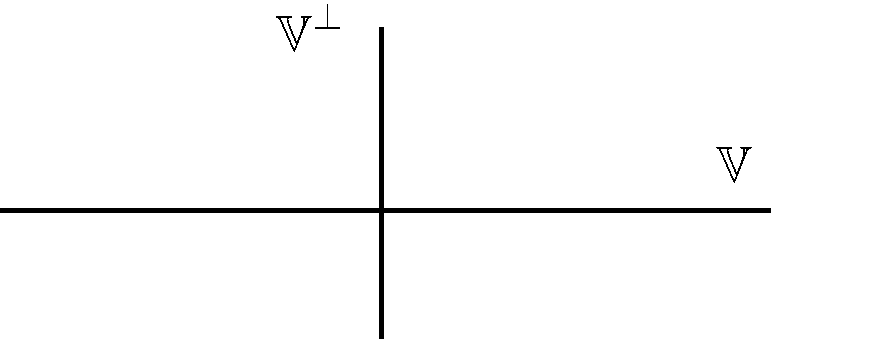
\includegraphics[width=2in]{figures/chap2_orthogonal_subspaces}		
\end{center}

\end{example}

\end{frame}

%----------------------------------
\begin{frame}\frametitle{Orthogonal Subspaces, cont.}
	
\begin{theorem}
Let $V$ and $W$ be subspaces of an inner product space $S$ (not necessarily Hilbert).  Then
\begin{enumerate}
  \item $V^{\perp}$ is a closed subspace of $S$
  \item $V \subset V^{\perp \perp}$  ($V = V^{\perp\perp}$ if $S$ is complete)
  \item If $V \subset W$ then $W^{\perp} \subset V^{\perp}$
  \item $V^{\perp\perp\perp} = V^{\perp}$
  \item If $x \in V \cap V^{\perp}$ then $x = 0$
  \item $\{0\}^{\perp} = S$ and $S^{\perp} = \{0\}$
\end{enumerate}
\end{theorem}
Prove one in class.
\end{frame}


%----------------------------------
\begin{frame}\frametitle{Inner Sum and Direct Sum}
\begin{definition}[Inner Sum] 
If $V$ and $W$ are linear subspaces then
\[ V + W = \{ x: x=v+w, v \in V \text{ and } w \in W\} \]
is the \underline{inner sum}.	
\end{definition}
\begin{definition}[Orthogonal Sum]
 If $V$ and $W$ are orthogonal subspaces then the sum
\[ V \oplus W = \{ x: x = v + w, v \in V \text{ and } w \in W\} \]
is called the orthogonal sum.	
\end{definition}
\begin{definition}[Disjoint Subspaces]
Two subspaces are said to be disjoint if
\[ V \cap W = \{ 0 \} \]	
\end{definition}

\end{frame}

%----------------------------------
\begin{frame}\frametitle{Inner Sum and Direct Sum, cont.}
\begin{lemma}
  Let $V + W$ be subspaces of $S$ and let $x \in V + W$ then the
  representation $x = v + w$ is unique iff $V + W$ are disjoint.
\end{lemma}
\begin{proof}
	($\Leftarrow$) Assume $V,W$ are disjoint but $x = v+w$
is not unique i.e. $x = v_1+w_1 = v_2+w_2$ where $v_1 \neq v_2$ and
$w_1 \neq w_2$.  This implies that $v_1 - v_2 = w_2 - w_1$ but $v_1 -
v_2 \in V$ and $w_2 - w_1 \in W$ since $V,W$ are subspaces.  Since $V
\cap W = \{ 0 \}$ we must have that $v_1 - v_2 = w_2 - w_1 = 0$ or
$v_1 = v_2$ and $w_1 = w_2$ which is a contradiction.
\end{proof}

\end{frame}

%----------------------------------
\begin{frame}\frametitle{Inner Sum and Direct Sum, cont.}
\begin{lemma}
  If $V$ and $W$ are orthogonal subspaces then the representation of
  $x \in V \oplus W$ is unique (i.e. $x = v+w$, where $v\in V$ and $w\in W$).
\end{lemma}
\begin{example}
Let $S = \mathbb{R}^2$, let $V =
\left\{\left( \begin{array}{c} \alpha \\ 0 \end{array} \right) :
  \alpha \in \mathbb{R} \right\}$, let $W = \left\{ \left( \begin{array}{c} 0
      \\ \alpha \end{array} \right) : \alpha \in \mathbb{R} \right\}$ Then
\[ \left(\begin{array}{c} 5 \\ 2 \end{array}\right) =
\left( \begin{array}{c} 5 \\ 0 \end{array} \right) +
\left( \begin{array}{c} 0 \\ 2 \end{array} \right) \] is a
\underline{unique} decomposition.
\end{example}
\end{frame}

%----------------------------------
\begin{frame}\frametitle{Difference between a Hamel basis and a Complete basis.}
\begin{definition}	
An orthonormal set of basis vectors $T = \{ p_i,
p_2, \ldots \}$ is said to be a compelte basisfor a Hilbert space $S$
if every $x \in S$ can be represented as
\[ x = \sum_{j=1}^{\infty}c_j p_j \]	
\end{definition}

\vfill

{\em Examples of complete bases:}
Fourier functions: $e^{j\omega t}$\\
Legendre \& Chebyshev polynomials

\vfill

{\em Difference:} A Hamel basis $\Rightarrow$ every $x$ can be
represented by a \underline{finite} representation.  A complete basis
allows functions through a limiting process.

\end{frame}


%%%%%%%%%%%%%%%%%%%%%%%%%%%%%%%%%%%%%%%%%%%%%%%%%%%%%%%%%%%%%%%%%%%%%%%
\section{Linear Operators}
\frame{\sectionpage}

%----------------------------------
\begin{frame}\frametitle{Operators and Transformations}
\begin{definition}[Linear Operator]	
	Let $\mathcal{L}:\mathbb{X}\to\mathbb{Y}$ be an operator from $\mathbb{X}$ to
$\mathbb{Y}$.  $\mathcal{L}$ is a \underline{linear operator} if
\begin{enumerate}
  \item $\mathcal{L}[\alpha x] = \alpha \mathcal{L}[x] \qquad \forall x \in \mathbb{X} \qquad \forall \alpha \in \mathbb{F}$
  \item $\mathcal{L}[x_1 + x_2] = \mathcal{L}[x_1] + \mathcal{L}[x_2], \qquad \forall x_1, x_2\in\mathbb{X}$
\end{enumerate}
\end{definition}

\end{frame}

%----------------------------------
\begin{frame}\frametitle{Examples of Linear Operators}
\begin{example}[Matrices]	
Operators from $\mathbb{C}^n$ to $\mathbb{C}^m$ are $m \times n$ matrices.
\[ A(\alpha x + \beta y) = \alpha Ax + \beta Ay \] 
A is a linear operator.
\end{example}

\begin{example}[Differential Equations with no input]
The differential equation $\dot{x} = Ax; \quad x(0) = x_0$
defines a linear operator from $\mathbb{R}^n$ to $L_2[0,T]$
\[
y(t) = \mathcal{L}[x_0] \text{ where } \mathcal{L}[x_0] = e^{At}x_0 
\]
\indent $\mathcal{L}$ is linear since 
\[ 
e^{At}(\alpha x_{01} + \beta  x_{01}) = \alpha e^{At}x_{01} + \beta e^{At}x_{02} 
\]
\end{example}


\end{frame}

%----------------------------------
\begin{frame}\frametitle{Examples of Linear Operators}
\begin{example}[Convolution]
Convolution is a linear operator from $L_{\infty}$ to
$L_{\infty}$ if $h(t) \in L_1[-\infty,\infty]$, i.e.
\[ y(t) = \mathcal{L}[x(t)] = \int_{-\infty}^{\infty} h(\tau)x(t - \tau)
d\tau \] 
\indent (Recall: for a system to be BIBO stable required
that $\int_{-\infty}^{\infty}|h(\tau)|d\tau <\infty$
\indent i.e. $h(t) \in L_1[-\infty,\infty]$)
\end{example}
\end{frame}

%----------------------------------
\begin{frame}\frametitle{Examples of Linear Operators}
\begin{example}[Fourier Transform]
\noindent (E4) The Fourier transform defines a linear operator from $L_2[-\infty,\infty]$ to $L_2[-\infty,\infty]$.\\
\[ X(j\omega) = \mathcal{L}[x(t)] \defeq \int_{-\infty}^{\infty} x(t)e^{-j\omega t}dt \]	
\end{example}

\vspace{1cm}
{\em There are many examples of linear operators!}
\end{frame}

%----------------------------------
\begin{frame}\frametitle{Range and Null Space of an Operator}
\begin{definition}[Range Space]
	Let $\mathcal{L}: \mathbb{X} \to \mathbb{Y}$ be a
linear operator.  The \underline{range space} (or \underline{image}) of $\mathcal{L}$ is 
\[
\mathcal{R}(\mathcal{L}) = \{ y \in \mathbb{Y} : y = \mathcal{L}[x] \text{ and } x \in \mathbb{X}\} \subseteq \mathbb{Y}
\]
\end{definition}
\begin{definition}[Null Space]
The \underline{Null space} or \underline{kernel} of $\mathcal{L}$ is
\[
\mathcal{N}(\mathcal{L}) = \{ x \in \mathbb{X} : \mathcal{L}[x] = 0 \} \subseteq \mathbb{X} 
\]	
\end{definition}
	
\end{frame}

%----------------------------------
\begin{frame}\frametitle{Example of Range and Null Space}
\begin{itemize}
\item Consider the matrix $A=\begin{pmatrix} 1 & 0 & 0\\ 0 & 0 & 0 \end{pmatrix}$ which defines a linear operator from $\mathbb{R}^3$ to $\mathbb{R}^2$.
\item Note that $y=Ax = 	\begin{pmatrix} 1 & 0 & 0 \\ 0 & 0 & 0 \end{pmatrix}\begin{pmatrix} x_1 \\ x_2 \\ x_3 \end{pmatrix} = \begin{pmatrix} x_1 \\ 0 \end{pmatrix}$.
\item Therefore, the range space is
	\[
	\mathcal{R}(A) = \left\{\begin{pmatrix}\alpha \\ 0 \end{pmatrix} : \alpha\in\mathbb{R} \right\} \subset \mathbb{R}^2.
	\]
\item Similarly, the null space is
	\[
	\mathcal{N}(A) = \left\{\begin{pmatrix}0 \\ \alpha \\ \beta \end{pmatrix} : \alpha, \beta\in\mathbb{R} \right\}\subset \mathbb{R}^3.
	\]
\end{itemize}
\end{frame}

%%%%%%%%%%%%%%%%%%%%%%%%%%%%%%%%%%%%%%%%%%%%%%%%%%%%%%%%%%%%%%%%%%%%%%%
\section{Projections}
\frame{\sectionpage}

%----------------------------------
\begin{frame}\frametitle{Projections}
\begin{itemize}
%\item This topic is probably the most important and useful topic covered in
%this class.  We will use it over and over.

\item Suppose that $V$ and $W$ are disjoint subspaces of $S$ such that $V + W = S$, i.e.
\[ x \in S \Rightarrow x = v + w\]
where $v \in V$ and $w \in W$ is a unique decomposition.

\item Define the linear operator $P:S\to V \subset S$ as 
\[ Px = P(v+w) = v \]

\item Note that $P(Px) = Pv = v$
\end{itemize}
	
\end{frame}

%----------------------------------
\begin{frame}\frametitle{Projections, cont.}
\begin{definition}[Projection Operator] 
Let $P: S \to S$ such that $P^2 = P$,
then $P$ is called a \underline{projection} operator or \underline{idempotent}.	
\end{definition}

\begin{example}
Let $P = \left( \begin{array}{cc} 1 & 0
    \\ 0 & 0 \end{array} \right)$, then $P\left( \begin{array}{c} x_1
    \\ x_2 \end{array} \right) = \left( \begin{array}{c} x_1 \\
    0 \end{array} \right)$\\
i.e. $P$ projects elements of $P$ onto the $x_1$ axis:

\begin{center}
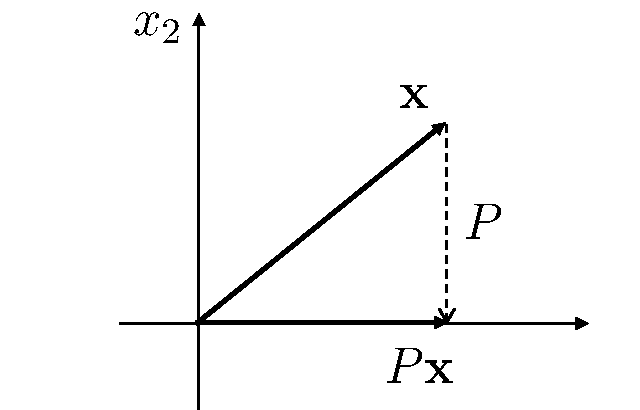
\includegraphics[width=2in]{figures/chap2_projection_1}
\end{center}

\end{example}
\end{frame}

%----------------------------------
\begin{frame}\frametitle{Projections, cont.}
\begin{example}
Truncation: let 
\[
(P_T x)(t) = \begin{cases} x(t), &\quad -T \leq t \leq T\\
0, &\quad \text{ otherwise }\end{cases}
\]
Then $P_T$ projects $x(t)$ onto its truncated function:\\

\begin{center}
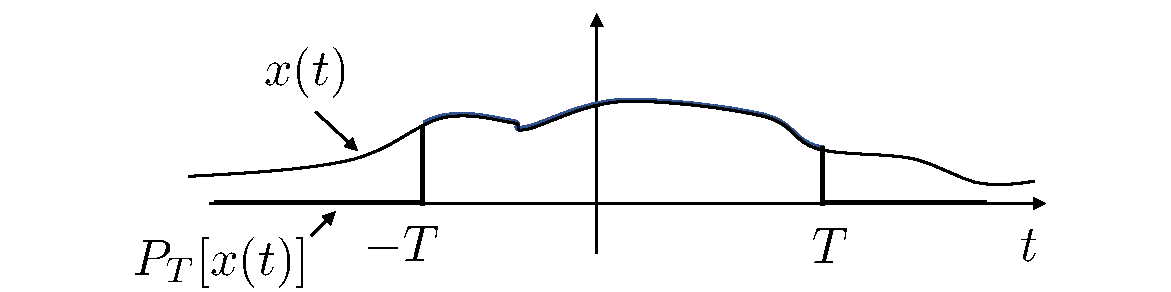
\includegraphics[width=4in]{figures/chap2_projection_2}	
\end{center}
\end{example}
\end{frame}

%----------------------------------
\begin{frame}\frametitle{Projections, cont.}
\begin{theorem}[Moon 2.7]
Let $P:S\to S$ be a projection operator, then
\[ 
S = R(P) + N(P) 
\]	
\end{theorem}
\begin{proof}
Homework problem.	
\end{proof}
\end{frame}

%----------------------------------
\begin{frame}\frametitle{Projections, cont.}
\begin{theorem}
	If $P:S\to S$ is a projection operator then so is $(I - P):S\to S$
\end{theorem}
\begin{proof}
\begin{flalign*}
  (I - P)^2 &= (I - P)(I - P) = \\
  &= I - P - P - P^2\\
  &= I - P - P + P\\
  &= I - P
\end{flalign*}	
\end{proof}
\end{frame}

%----------------------------------
\begin{frame}\frametitle{Projections, cont.}
\begin{itemize}
\item Note that if $P:S\to V$ and $I-P:S\to W$ then $V$ and $W$
are disjoint and $S=V+W$ since 
\[
x = \underbrace{Px}_{\in V} + \underbrace{(I-P)x}_{\in W}.
\]

\item $V$ and $W$ are disjoint.  If not, then $\exists x_0 (\neq 0) \in S$ such that 
\begin{flalign*}
Px_0 &= (I - P)x_0 = x_0 - Px_0\\
2Px_0 &= x_0\\
\Rightarrow Px_0 &= \frac{1}{2}x_0\\
\text{ and } P^2x_0 &= \frac{1}{4}x_0 = \frac{1}{2}x_0 \Leftrightarrow x_0 = 0
\end{flalign*}

\end{itemize}
\end{frame}

%----------------------------------
\begin{frame}\frametitle{Projections, cont.}

\begin{definition}[Orthogonal Projection]
If $V$ and $W$ are orthogonal then $P$ is an \underline{orthogonal projection}\\
\end{definition}

\begin{theorem}
	$P$ is an orthogonal projection iff $R(P) \perp N(P)$
\end{theorem}
\end{frame}

%----------------------------------
\begin{frame}\frametitle{Applications to Engineering}
Given a point $x \in S$, suppose that we want to approximate $x$ by a
point in $\mathbb{V}\subset S$ (assuming $x \notin \mathbb{V}$) then
we want to find the point in $\mathbb{V}$ that is closest to $x$.\\

\begin{center}
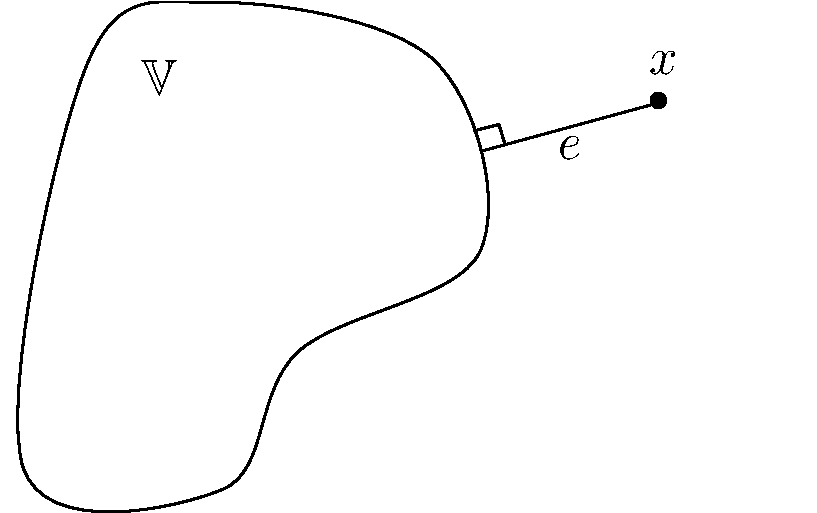
\includegraphics[width=2in]{figures/chap2_projection_on_set}
\end{center}

This is given by the orthogonal projection of $x$ onto $\mathbb{V}$.  i.e. $\iprod{ e,v} = 0 \qquad \forall v \in \mathbb{V}$

\end{frame}

%----------------------------------
\begin{frame}\frametitle{Applications to Engineering}
Let $\nbf$ be a unit vector in $\mathbb{R}^3$ (i.e., $\norm{\nbf}=1$), then 
\[
\Pi_\nbf^\perp \defeq \nbf \nbf^\top
\]
is a projection operation.  Geometrically $\Pi_\nbf^\perp x = \nbf \nbf^\top x$ find the projection of $x$ along the unit vector $\nbf$

Also 
\[
\Pi_\nbf = I-\nbf\nbf^\top
\]
is a projection operator.  Geometrically, $\Pi_\nbf x$ projections $x$ onto the 2D space that is orthogonal to $\nbf$.

\end{frame}

%----------------------------------
\begin{frame}\frametitle{The Projection Theorem}
\begin{theorem}
Let $\mathbb{S}$ be a Hilbert space and let $\mathbb{V}$ be a closed subspace of $\mathbb{S}$.  For any $x \in \mathbb{S}$ there exists a unique $v_0 \in \mathbb{V}$ closest to $x$;  i.e. $\norm{ x - v_0 } \leq \norm{ x - v } \quad \forall v \in \mathbb{V}$.\\


\vspace{1cm}

Furthermore $v_0$ minimizes $\norm{ x - v_0 }$ iff $x - v_0$ is orthogonal to $\mathbb{V}$.	
\end{theorem}
	
\end{frame}

%----------------------------------
\begin{frame}\frametitle{The Projection Theorem, proof}

{\bf Step 1.  Show that $v_0$ exists.}

Assume $x \notin \mathbb{V}$ and let $\delta = \inf_{v \in \mathbb{V}} \norm{ x - v } $
We need to show that in fact $\exists v_0 \in \mathbb{V}$ such that $\norm{ x - v_0 } = \delta$\\

Let $\{v_i\}$ be a sequence in $\mathbb{V}$ such that $\norm{ x - v_i } \to \delta $ and show that $\{ v_i \}$ is Cauchy.

\vfill
Need parallelogram law:
\[ 
\norm{ x + y }^2 + \norm{ x - y }^2 = 2\norm{ x }^2 + 2\norm{ y }^2.
\]
\vfill

Consider
\begin{multline*}
\norm{ (v_j - x) + (x - v_i) }^2 + \norm{ (v_j - x) - (x-v_i) }^2 \\
	= 2\norm{ (v_j-x) }^2 + 2\norm{ x - v_i }^2
\end{multline*}
\[ 
\Rightarrow \norm{ v_j - v_i }^2 = 2\norm{ v_j - x }^2 + 2\norm{ x - v_i }^2 - 4\norm{ \frac{(v_j + v_i)}{2} - x }^2
\]

\end{frame}

%----------------------------------
\begin{frame}\frametitle{The Projection Theorem, proof}
$v_i,v_j \in \mathbb{V} \quad \Rightarrow\quad \frac{v_j+v_i}{2} \in \mathbb{V} \quad\Rightarrow\quad\norm{ \frac{(v_j-v_i)}{2} - x }^2 \geq \delta^2$

\[ \Rightarrow \norm{ v_j - v_i }^2 \leq 2\norm{ v_j - x }^2 + 2\norm{ v_i - x }^2 - 4\delta^2 \]
But $\norm{ v_j - x } \to \delta$
\[ \Rightarrow \norm{ v_j - v_i } \to 0 \] and is therefore Cauchy.

\vfill

Since $\mathbb{V}$ is a Hilbert space
\[ v_i \to v_0 \in \mathbb{V}. \]

\vfill

Note that this proof is not constructive, i.e. it doesn't tell you how to construct the sequence $\{v_i\}$.
\end{frame}

%----------------------------------
\begin{frame}\frametitle{The Projection Theorem, proof}
{\bf Step 2.  Show that $v_0 = \arg\min_{v\in\mathbb{V}} \norm{ x - v } \Rightarrow x - v_0 \perp \mathbb{V}$}.

Proof by contradiction. Suppose that $x-v_0$ is not perpendicular to $\mathbb{V}$.  Then there exists a $v \in \mathbb{V}$ such that 
\[ \iprod{ x - v_0, v} = \delta \neq 0 \]
and w.l.o.g. (why?) let $\norm{ v } = 1$

\vfill

Let $z = v_0 + \delta v \in \mathbb{V}$ then 
\begin{flalign*}
\norm{ x - z }^2 = \norm{ x - v_0 - \delta v }^2 &= \norm{ x - v_0 }^2 - 2 Re \iprod{ x - v_0, \delta v} + \norm{ \delta v }^2 \\
&= \norm{ x - v_0 }^2 - 2 \delta^2 + \delta^2 < \norm{ x - v_0 }^2
\end{flalign*}
which is a contradiction since $v_0$ is the minimizer.
\end{frame}


%----------------------------------
\begin{frame}\frametitle{The Projection Theorem, proof}

{\bf Step 3.}
Suppose $(x - v_0) \perp \mathbb{V}$ then $\forall v \in \mathbb{V}$ such that $v \neq v_0$
\begin{align*}
\norm{ x - v }^2 &= \norm{ x - v_0 + v_0 - v }^2\\
&= \norm{ x - v_0}^2 + 2 Re \iprod{ x - v_0, v_0 - v} + \norm{ v_0 - v }^2\\
&= \norm{ x - v_0 }^2 + \norm{ v_0 - v }^2\\
&> \norm{ x - v_0 }^2
\end{align*}

{\bf Step 4. Uniqueness}
Same as proof on page 25 of notes.
	
\end{frame}

%----------------------------------
\begin{frame}\frametitle{Closed Subspace}
\begin{theorem}[Moon Theorem 2.10]
Let $\mathbb{V}$ be a closed subspace of a Hilbert space $\mathbb{S}$, then
\begin{flalign*}
\mathbb{S} &= \mathbb{V} \oplus \mathbb{V}^{\perp}\\
\mathbb{V} &= \mathbb{V}^{\perp \perp}
\end{flalign*}
\end{theorem}
\begin{proof}
In book.	
\end{proof}
	
\end{frame}




%%%%%%%%%%%%%%%%%%%%%%%%%%%%%%%%%%%%%%%%%%%%%%%%%%%%%%%%%%%%%%%%%%%%%%%
\section{Gram Schmidt Orthogonalization}
\frame{\sectionpage}


%----------------------------------
\begin{frame}\frametitle{Application:  Gram Schmidt Orthogonalization}
\noindent Given a set $T = \{ p_1, \ldots, p_n\}$

\noindent Find a set $T' = \{q_1, \ldots, q_n'\} \qquad n' \leq n$ such that
\[ span(T') = span(T) \text{ and } <q_i,q_j> = \delta_{ij} \]

\begin{description}
\item[Step 1.]
Normalize the First Vector
\[ q_1 = \frac{p_1}{\norm{ p_1 }} \qquad \text{ (i.e. } \iprod{ q_1,q_1 }=1 \text{ ) } \]
\end{description}
\end{frame}

%----------------------------------
\begin{frame}\frametitle{Application:  Gram Schmidt Orthogonalization, cont}

\begin{description}
\item[Step 2.]	
Let $e_2$ be $p_2$ minus the projection of $p_2$ on $q_1$
i.e.
\[ e_2 = p_2 - \iprod{ p_2, q_1} q_1 \]

\begin{center}
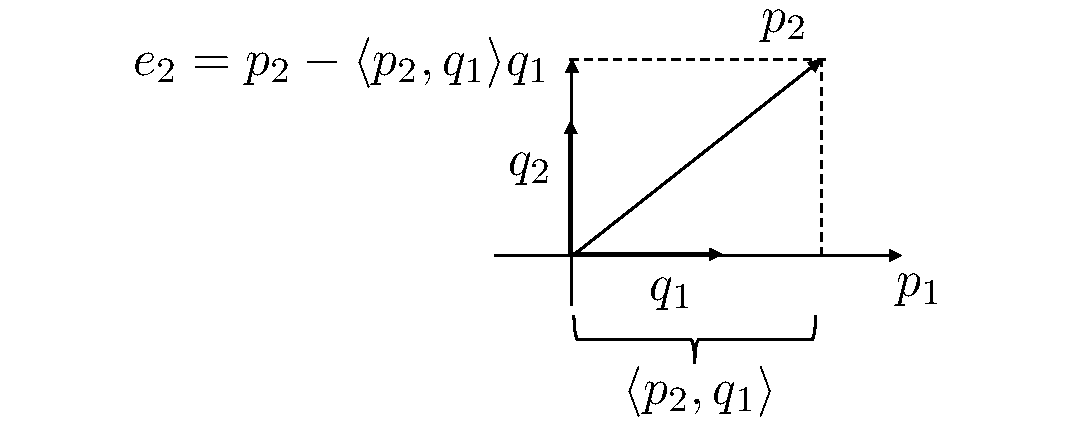
\includegraphics[width=4in]{figures/chap2_gram_schmidt}
\end{center}

Then normalize $e_2$:
\[ q_2 = \frac{e_2}{\norm{ e_2 }} \]
\end{description}
\end{frame}

%----------------------------------
\begin{frame}\frametitle{Application:  Gram Schmidt Orthogonalization, cont}

\begin{description}
\item[Step 3.]
Let $e_k$ be $p_k$ minus the projection of $p_k$ on $q_1, \ldots, q_{k-1}$:
\[ e_k = p_k - \sum_{j=1}^{k-1}\iprod{ p_k, q_j} q_j \Rightarrow q_k = \frac{e_k}{\norm{ e_k }} \]
\end{description}
\end{frame}

%----------------------------------
\begin{frame}\frametitle{Example: Gram Schmidt Orthogonalization}
Given the set
\[
T = \{ p_1, p_2, p_3 \} \defeq \left\{ \begin{pmatrix} 2 \\ 0 \\ 0 \end{pmatrix}, \begin{pmatrix}1 \\ 2 \\ 0 \end{pmatrix}, \begin{pmatrix} 1 \\ 2 \\ 3 \end{pmatrix} \right\}
\]	
find a set $T'=\{q_1, q_2, q_3\}$ where the vectors in $T'$ are orthonormal and $\text{span}(T)=\text{span}(T')$.

\vfill

\[
q_1 = \frac{p_1}{\norm{p_2}} = \frac{\begin{pmatrix} 2 \\ 0 \\ 0 \end{pmatrix}}{2} = \begin{pmatrix} 1 \\ 0 \\ 0 \end{pmatrix}.
\]

\end{frame}

%----------------------------------
\begin{frame}\frametitle{Example: Gram Schmidt Orthogonalization, cont.}

\begin{align*}
e_2 &= p_2 - \iprod{p_2, q_1} q_1 \\
    &= \begin{pmatrix} 1 \\ 2 \\ 0 \end{pmatrix} - \begin{pmatrix} 1\\2\\0\end{pmatrix}^\top\begin{pmatrix}1\\0\\0\end{pmatrix}\begin{pmatrix}1\\0\\0\end{pmatrix} \\
    &= \begin{pmatrix} 1 \\ 2 \\ 0 \end{pmatrix} - 1\cdot\begin{pmatrix}1\\0\\0\end{pmatrix} \\
    &= \begin{pmatrix}0\\2\\0\end{pmatrix}
\end{align*}
Therefore
\(
q_2 = \frac{e_2}{\norm{e_2}} = \frac{\begin{pmatrix}0\\2\\0\end{pmatrix}}{2} = \begin{pmatrix}0\\1\\0\end{pmatrix}
\)

\end{frame}

%----------------------------------
\begin{frame}\frametitle{Example: Gram Schmidt Orthogonalization, cont.}

\begin{align*}
e_3 &= p_3 - \iprod{p_3, q_1} q_1 -\iprod{p_3, q_2}q_2 \\
    &= \begin{pmatrix} 1 \\ 2 \\ 3 \end{pmatrix} - \begin{pmatrix} 1\\2\\3\end{pmatrix}^\top\begin{pmatrix}1\\0\\0\end{pmatrix}\begin{pmatrix}1\\0\\0\end{pmatrix} - \begin{pmatrix} 1\\2\\3\end{pmatrix}^\top\begin{pmatrix}0\\1\\0\end{pmatrix}\begin{pmatrix}0\\1\\0\end{pmatrix} \\
    &= \begin{pmatrix} 1 \\ 2 \\ 3 \end{pmatrix} - 1\cdot\begin{pmatrix}1\\0\\0\end{pmatrix}  - 2\cdot\begin{pmatrix}0\\1\\0\end{pmatrix} \\
    &= \begin{pmatrix}0\\0\\3\end{pmatrix}
\end{align*}
Therefore
\(
q_3 = \frac{e_3}{\norm{e_3}} = \frac{\begin{pmatrix}0\\0\\3\end{pmatrix}}{3} = \begin{pmatrix}0\\0\\1\end{pmatrix}
\)

\end{frame}

%----------------------------------
\begin{frame}\frametitle{Example: Gram Schmidt Orthogonalization, cont.}

Therefore, the Gram Schmidt orthonormalization of 
\[
T = \{ p_1, p_2, p_3 \} \defeq \left\{ \begin{pmatrix} 2 \\ 0 \\ 0 \end{pmatrix}, \begin{pmatrix}1 \\ 2 \\ 0 \end{pmatrix}, \begin{pmatrix} 1 \\ 2 \\ 3 \end{pmatrix} \right\}
\]	
is
\[
T' = \{q_1, q_2, q_3\} = \left\{ \begin{pmatrix} 1 \\ 0 \\ 0 \end{pmatrix}, \begin{pmatrix}0 \\ 1 \\ 0 \end{pmatrix}, \begin{pmatrix} 0 \\ 0 \\ 1 \end{pmatrix} \right\}.
\]

\vfill

Note that $\text{span}(T)=\text{span}(T')$.

\end{frame}


\end{document}
